\documentclass[11pt, a4paper, norsk]{NTNUoving}
\usepackage[utf8]{inputenc}
\usepackage[T1]{fontenc}
\usepackage{mathrsfs}
\newcommand{\RomanNumeralCaps}[1]
{\MakeUppercase{\romannumeral #1}}


\ovingnr{1}    % Nummer på innlevering
\semester{Haust 2022}
\fag{TMA4120}
\institutt{Institutt for matematiske fag}

\begin{document}
\section*{6.1}

\begin{oppgave} % oppgave
  $\mathscr{L}[2t+8]=\frac{2}{s^{2}}+\frac{8}{s}$
\end{oppgave}
\begin{oppgave}[12] La
  \[
f(t) =
     \begin{cases}
      t &\quad 0<t<1\\
      1 &\quad 1\leq t < 2 \\
      0 &\quad \text{ellers}
     \end{cases}
    \]
   Det gir
   \[
 \mathscr{L}[f(t)] =
     \begin{cases}
      \mathscr{L}[t] &\quad 0<t<1\\
      \mathscr{L}[1] &\quad 1\leq t < 2 \\
      \mathscr{L}[0] &\quad \text{ellers}
     \end{cases}
\]\[\Rightarrow \mathscr{L}[f(t)]=
     \begin{cases}
      \frac{1}{s^{2}} &\quad 0<t<1\\
      \frac{1}{s} &\quad 1\leq t < 2 \\
      0 &\quad \text{ellers}
     \end{cases}
    \]
\end{oppgave}
\begin{oppgave}[23]
  Bruker definisjonen av Laplace-transformasjonen, i lag med variabelbytte $r=ct$.
  \[
\mathscr{L}[f(ct)]=\int_{0}^{\infty}f(ct)e^{-st}dt=\int_{0}^{\infty}f(r)e^{-(s/c)r}\frac{dr}{c}=\frac{1}{c}F(s/c)
 \]
 Dette resultatet kan vi bruke til å finne
 \[
   \mathscr{L}[\cos(\omega t)]=\frac{1}{\omega}F(s/\omega)=\frac{1}{\omega}\frac{s/\omega}{(s/\omega)^{2}+1} =\frac{s}{s^{2}+\omega^{2}}
 \] der vi bruker
 \[
   \mathscr{L}[\cos(t)]=F(s)=\frac{s}{s^{2}+1}
 \]
\end{oppgave}
\begin{oppgave}[26]
  \[
    f(t)= \mathscr{L}^{-1}\left[\frac{5s+1}{s^{2}+25}\right]=
     \mathscr{L}^{-1}\left[\frac{5s}{s^{2}+5^{2}}\right]+\mathscr{L}^{-1}\left[\frac{1}{s^{2}+5^{2}}\right]
    = 5\cos(5t)-\sin(5t)
  \]
\end{oppgave}
\begin{oppgave}[36]
  Bruker eksponentialdefinisjonen til $\sinh(t)$, samt skift langs $s$-aksen.
  \[
    \mathscr{L}[\sinh(t)\cos(t)]=\frac{1}{2} \mathscr{L}[e^{t}\cos(t)-e^{-t}\cos(t)] = \frac{1}{2}\left[\frac{s-1}{(s-1)^{2}+1}-\frac{s+1}{(s+1)^{2}+1}\right]
  \]
  Dette utrykket kan ved litt bokføring forenklest til
  \[
    \mathscr{L}[\sinh(t)\cos(t)]=\frac{s^{2}-2}{s^{4}+4}
  \]
\end{oppgave}
\begin{oppgave}[40]
  Starter med å bearbeide brøken.
  \[
    \frac{4}{s^{2}-2s-3}=\frac{4}{s^{2}-2s+1-4}=\frac{4}{(s-1)^{2}-2^{2}}
  \]
  Det gir
  \[
    f(t)= \mathscr{L}^{-1}\left[\frac{4}{(s-1)^{2}-2^{2}}\right]=2e^{t}\sinh(2t)
  \]
  Har brukt skift langs $s$-aksen, samt kjennskap om Laplacetransformen til $\sinh(\omega t)$.
\end{oppgave}
\section*{6.2}
\begin{oppgave}[4]
  Laplacetransformerer likningen og får
  \[
    s^{2}Y+9Y=\frac{10}{s+1}
  \]
  Løser så for $Y$
  \[
    Y = \frac{10}{(s+1)(s^{2}+9)}
  \]
  Ved delbrøkoppspaltning kan vi forenkle dette, og finne invers Laplacetransform.
  \[
    y(t)= \mathscr{L}^{-1}\left[\frac{1-s}{s^{2}+9}-\frac{1}{s+1}\right]
        = \frac{1}{3}\sin(3t)-\cos(3t)-e^{t}
  \]
\end{oppgave}
\begin{oppgave}[13]
  Laplacetransformerer likningen:
  \[
    sY-y(0)-6Y=0\Rightarrow Y=\frac{y(0)}{s-6}
  \]
  Dette kan vi enkelt finne inverstransformen av.
  \[
    y(t)=y(0)e^{6t}
  \]
  Bruker så initialverdien:
  \[
    y(-1)=y(0)e^{-6}=4\Rightarrow y(0)=4e^{6}
  \]
  Kan så løse for $y(t)$:
  \[
    y(t)=4e^{6t+6}
  \]
\end{oppgave}
\newpage
\section*{6.3}
\begin{oppgave}[8]
  Har brukt python til å lage en figur:

  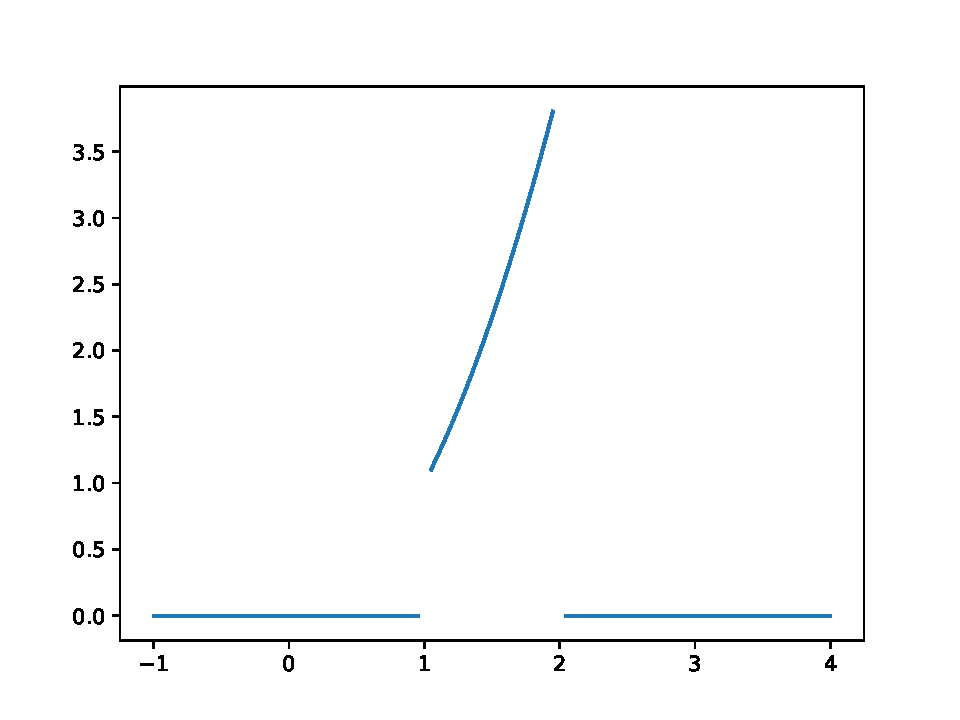
\includegraphics[scale=0.5]{6.2.8.pdf}

  Vi kan konstruere denne funksjonen med stegfunksjoner. Vi vil at stegfunksjonene skal være ``på'' i intervallet $1<t<2$, og 0 ellers. Dette oppnår vi slik:
  \[
    f(t)=t^{2}(u(t-1)-u(t-2))
  \]
  Kan finne Laplacetransformen ved å bruke definisjonen
  \[
    \mathscr{L}[f(t)]=\int_{0}^{\infty}f(t)e^{-st}dt= \int_{1}^{2}te^{-st}dt
  \]
  Gjennon noen steg med delvis integrasjon blir dette
  \[
    \mathscr{L}[f(t)]=\frac{2e^{-s}}{s^{3}}-\frac{2e^{-2s}}{s^{3}}
    +\frac{2e^{-s}}{s^{2}}-\frac{4e^{-2s}}{s^{2}}
    +\frac{e^{-s}}{s}-\frac{4e^{-2s}}{s}
  \]
\end{oppgave}
\begin{oppgave}[15]
  Ser at vi kan bruke t-skift for å finne inverstransformen.
  \[
    \mathscr{L}^{-1}\left[\frac{e^{-2s}}{s^{6}}\right]= \mathscr{L}^{-1}\left[e^{-2s} \mathscr{L}\left[\frac{t^{5}}{5!}\right]\right]=\frac{(t-2)^{5}}{5!}u(t-2)
  \]
  Lager en enkel skisse i python.

  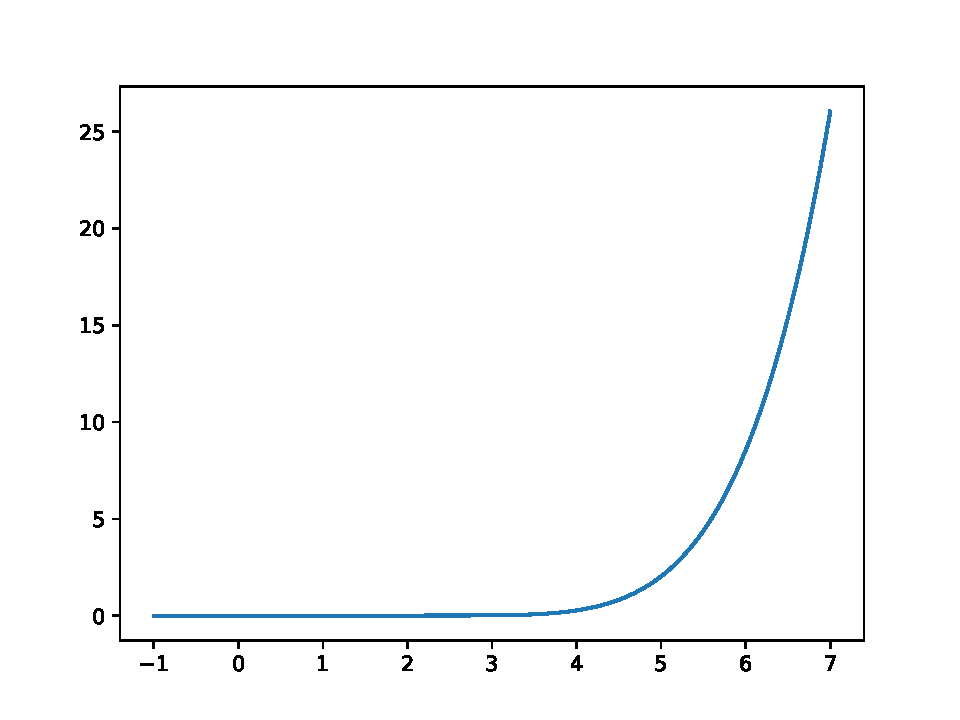
\includegraphics[scale=0.5]{6.3.15.pdf}
\end{oppgave}
\begin{oppgave}[25]
  Gitt at y er løst utenfor $0<t<1$, fokuserer vi på å løse difflikningen for dette intervallet. Bruker Laplacetransformen og får
  \[
    s^{2}Y+2+Y=\frac{2}{s^{2}}\Rightarrow Y=\frac{2}{s^{2}(s^{2}+1)}-\frac{4}{s^{2}+1}
  \]
  Ved delbrøkoppspaltning kan dette forenklest til
  \[
    Y=\frac{2}{s^{2}}-\frac{4}{s^{2}+1}
  \]
  Dette kan vi finne inverstransformen til, og det gir
  \[
    y(t)=2t-4\sin(t)\text{   , } 0<t<1
  \]
\end{oppgave}
\end{document}
